In this section we highlight how the UC experiment is encoded in NomosUC.
Recall from Section~\ref{sec:base} that linear session types impose constraints on what forms of communication can be captures, and pose challenges to supporting 
a dynamic number of protocol parties, or functionalities, at runtime. 
Combined with providerless channels, we create the \partywrapper that runs protocol parties in a sandbox and manages their communication with \F, \A, and \Z.
We validate our encoding of the UC experiment by realizing a critical result from the UC literature, the Dummy Lemma, which highlights the degree to which NomosUC captures the flexibility and modularity of the UC ITM model. 
\todo{I don't know what the right wording is here but I think Andrew would understand the point I'm trying to make. The dummy lemma is a convenience thing but being able
to express it simply counts for something.}
Finally we cover to important operators, composition and multisession, which allow us to prove the full composition theorem of UC in NomosUC.

%In this section, we explain in detail our encoding of the UC security definition into Nomos-UC.
%Recall from Section~\ref{sec:background} that the UC security definition $\F_1 \xrightarrow{\pi} \F_2$ says we can realize some desired application $\F_2$ with a protocol $\pi$ that uses $\F_1$.
%More generally, we define UC realization in terms of an indistinguishability relation between two experiments: the real-world featuring the execution of $\pi$ with $\F_1$, and an ideal-world execution of $\F_2$ with an ideal protocol $\idealP$ that relays inputs/outputs directly to/from $\F_2$.%
%\footnote{This ideal protocol $\idealP$ is also the identity, since we can easily show $\F \xrightarrow{\idealP} \F$ for any functionality $\F$.}
%Below, we introduce how the UC experiment is defined in NomosUC, and then provide a composition operator $\circ$ for protocols and simulators that satisfies Theorem~\ref{thm:singlecomp}.

\subsection{The UC Experiment}
%The UC experiment is an execution of protocol parties and an ideal functionality, reacting to input by an adversary \A or the environment \Z.
The type definition of \inline{execUC} is straightforward \todo{once we have clarity on the intro and type system section length we can include the typedef of here, it's not very interesting imo}. 
It is parameterized by at least one virtual token type, depending on the protocol in question, to allow for sandboxing of other processes (usually by the adversary or environment) and message types specified by the protocol in question. 
Its only functional parameters are the security parameter $k$ and a random bit string $r$. 
It offers the type \m{execout}:
{\centering
\parbox{0cm}{
\begin{tabbing} 
 $\m{execout}[a] = \textcolor{red}{\getpot^n} \echoice{\mb{exec}: $\=$ \ichoice{ \mb{out}: Bit \product 1}}$ 
 \end{tabbing}}
}
The spawning procss for \m{execUC} provides it $n$ import tokens before the experiment starts. 
NomosUC forces us to be explicit in the polynomials used when checking a polynomial bound in the type system, and, as long as \m{execUC} is provided a number of tokens $n \in poly(k)$, Theorems~\ref{thm:global_ppt} and \ref{thm:preservation} guarantee that the experiment terminates in $poly(k)$. We can conclude that every process in the experiment is also running time polynomial in $k$.  

%\begin{figure*}
%\begin{lstlisting}[basicstyle=\footnotesize\BeraMonottFamily, mathescape, frame=single]
%$\nproc$ execUC[K][p2f,f2p][z2p,p2z][a2p,p2a][f2a,a2f]{p2fn,f2pn}{z2pn,p2zn}{a2pn,p2an}{f2an,a2fn}{n}: 
%  (k: Int), (rng: [Bit]) |- ($\$$d: execout)
%\end{lstlisting}
%\caption{Type definition for \m{execUC} with no virtual tokens.}
%\label{fig:execuc}
%\end{figure*}

Recall that providerless channels mean that all code is wrapped by processes that manage communication with the outside world. 
In \m{execUC}, the shared part of providerless channels are spawned and passed to wrapped instances of \Z, \A, and the \partywrapper (see Figure~\ref{fig:newpandq}). 
For example, channele between \Z and \A are spawned below and passed to \Z
\begin{lstlisting}[basicstyle=\footnotesize\BeraMonottFamily, mathescape]
#z_to_a $\leftarrow$ channel_init[$\tp{K}$][$\tp{z2a}$]{$\tp{z2an}$}
#a_to_z $\leftarrow$ channel_init[$\tp{K}$][$\tp{a2z}$]{$\tp{a2zn}$}
$\tg{...}$
$\$$z <- Env[K] k rng #z_to_p #p_to_z #z_to_a #a_to_z ;
\end{lstlisting}
The import parameters $\tp{z2an}$ and $\tp{a2zn}$ (the import amount) are type parameters to \inline{execUC}.
%When processes are spawned, their shell codes correctly connect the channel endpoints internally.
%We point out that process definitions for \Z, \A, \F, and $\Pi$ are not passed as parameters to \inline{execUC} because NomosUC currently doesn't support passing them as parameters.

The environment, \Z, is the first spawned process and offers the type \m{EtoZ} (below) on \inline{$\$$z} to \m{execUC}.
\Z sends an \mb{init} message with the list of corrupt parties and an SID (a user-defined type), and on \mb{start}, along with $n$ import tokens, \Z begins with the execution.
It concludes with a output \mb{Bit} to \m{execUC}.
{\centering
\parbox{0cm}{
\begin{tabbing}
 $\m{EtoZ}[a] = \textcolor{red}{\getpot^n} \ichoice{\mb{init}: $\=$ SID[a] \arrow [PID] \arrow$ \\
\>$\echoice{\mb{start} \arrow \ichoice{\mb{out}: Bit \arrow 1}}}$
 \end{tabbing}}
}
The output bit, \Z's guess of which world it is in, forms the basis of the definition of indistinguishability.

%\begin{figure*}[t]
%\begin{lstlisting}[basicstyle=\scriptsize\BeraMonottFamily, frame=single, mathescape, caption={The process definition of the \msf{execUC} function.}]
%$\Stype$ Bit{n} = <{n}| &{ exec: +{out : Bit $\rightarrow$ 1}} ;
%
%$\tb{proc}$ execUC[$\tp{K}$][$\tp{K1}$][$\tp{sid}$][$\tp{p2f,f2p}$][$\tp{z2p,p2z}$][$\tp{a2p,p2a}$][$\tp{a2f,f2a}$]{$\tp{p2fn,f2pn}$}{$\tp{p2zn,z2pn}$}{$\tp{a2pn,p2an}$}{$\tp{a2fn,f2an}$} :
%  (k: $\tgr{int}$), (r: [Bit]) |- ($\$$d: Bit)
%\end{lstlisting}
%\label{lst:execuc}
%\end{figure*}

\subsection{The \partywrapper}
\begin{figure}
	\centering
	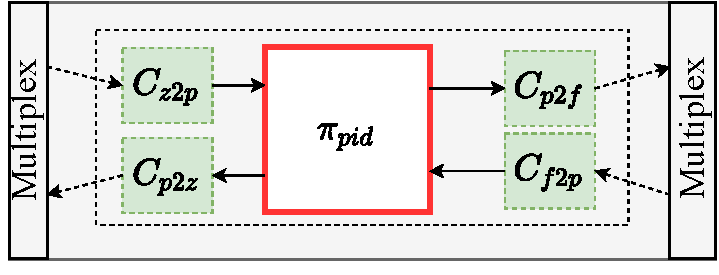
\includegraphics[scale=0.5]{figures/singleshellmultiplex.pdf}
	\caption{This is the \partywrapper that routes messages to the correct internally runnint protocol party. This figure shows how one protoco party (dotted box) is instantiated within it. The party $\pi_{pid}$ is shell code akin to Figure~\ref{fig:newpandq}.}%\snote{Updated caption to say it's multiplexer with one instance. The reason I don't want to include another instance is that I couldn't figure out a way to add it and expand the diagram horizontally. It will leave so much white space on the sides if I add a new party and will take up much more vertical space which we need to cut down on anyway.}}
	\label{fig:singlemultiplex}
	\vspace{-3mm}
\end{figure}
As a result of using channels, supporting dynamic parties requires new channels and to be connected to the rest of the experiment.
We use the \partywrapper to handle spawning parties, creating their channels, and connectint them to the rest of the experiment.
Instead of parties directly connected to \F and \Z through a providerless channels, the \partywrapper runs them virtually, internally, and presents a consistent ``real'' view to them. 
In turn, the \partywrapper is connected by single channels to \F, \Z, and \A, and it routes communication to/from the appropriate protocol party. 
In Figure~\ref{fig:singlemultiplex}, we see a wrapped protocol party, with its generated processes, inside the \partywrapper 

One tradeoff with the \partywrapper design is that the import sent to it by \F, \Z, and \A must be constant, because they each communicate with it over a single providerless channel. The protocol parties still receive virtual tokens according to their type. 
We don't see this as a downside of the approach as tight runtime constraints are not an intended goal of NomosUC or the UC framework.

The \partywrapper forces \F to also be wrapped to multiplex communication from the \partywrapper. 

\subsection{Emulation}
The central security definition in UC is indistinguishability between the real and ideal world experiments.
In NomosUC, we define the term \textit{well-matched} to mean the configuration resulting from a PPT term $e$ connected to another term $e'$ in well-typed, and we denote it as: $e \leftrightarrow e'$.
The term allows us to quantify statements over only adversaries and environments whose types match the protocol/functionality in question when reasoning about emulation. 

We define indistinguishability in terms of te ensemble of distributions of the output bit of the partial term $\m{execUC}\ \pi\ \F$ over all possible bitstrings and security parameters using the standard way of statistical distribution.  

%We define the output bit of the partial term of \inline{execUC}, for a specific $\pi$ and \F, as an ensemble of distributions over all possible random bitstrings and security parameters.
%Emulation, then, is about the ensembles created by two UC executions being computationally indistinguishable from each other.
%We define indistinuishability between ensembles in a standard way using \textit{statistical distance}: $\mathcal{D}_{1,k} sim \mathcal{D}_{2,k}$ if their statistical distance is at most $negl{k}, \forall k$.
%\begin{definition}[Indistinguishability]\label{def:distance}
%Two ensembles $\mathcal{D}_{1,k}, \mathcal{D}_{2,k}$ are indistinguishable, $\mathcal{D}_{1,k} \sim \mathcal{D}_{2,k}$, if their statistical distance is at most $negl(k), \forall k$.
%\end{definition}

UC emulation combines the UC execution with indistinguishability resulting in the following NomosUC emulation definition.
\begin{definition}[Emulation]\label{def:emulation}
If two protocols $(\pi, \F_1)$, $(\phi, \F_2)$, which we refer to only by \PI and $\phi$, emulated each other, then $\forall \A$ well-matched with \PI, there must $\exists \Sim$ well-matched with $\phi$ s.t. $\forall \Z$ : $\msf{execUC}(\pi, \F_1, \Z, \A)$ $\approx$ $\msf{execUC}(\phi, \F_2, \Z, \Sim)$:

\begin{mathpar}
	\footnotesize
	\inferrule*[right=emulate]
	{
		\pi : \Delta_1'[\Tokentypes][\mathrm{T}_{\pi}] \semi \phi : \Delta_2'[\Tokentypes][\mathrm{T}_{\phi}] \semi \\
		\forall \A \ | \ \Delta_4[\Tokentypes][\mathrm{T}_{\A}] \vdash \A :: \Delta_3', \ \langle \A \leftrightarrow \pi \rangle \\
		\Rightarrow \exists \ (\Delta_3[\Tokentypes][\mathrm{T}_{\Sim}] \vdash \Sim_\A :: \Delta_3') \ | \ \langle \Sim_\A \leftrightarrow \phi \rangle \\
		\Rightarrow \forall \Z  \; \msf{execUC} \ \pi\ \F_1\ \Z\ \A \approx\ \msf{execUC} \ \phi\ \F_2\ \Z\ \Sim_\A
	}
	{
		% EMULATION DEFINITION
		\lambda \A \, . \, \Sim_\A \vdash (\pi, \F_1) \sim (\phi, \F_2)
	}
\end{mathpar}
\end{definition}
Given two protocol $\pi$ and $\phi$, for all \A of type $\Delta_3'$ there is a simulator $\Sim$ also of type $\Delta_3'$ that is well-matched with $\phi$. For all environments matched with $\A$ and $\Sim$,
the two experiments should be indistinguishable.

An important validation of our approach is the the Dummy Lemma~\ref{thm:dummythicclemma} which shows that a simulator, \DS, for the dummy adversary satisfies the emulation definition for all adversaries \A. 
\begin{theorem}[Dummy Lemma]\label{thm:dummythicclemma}
If \ $\exists \DS$ s.t. $ \DA, \DS \vdash \F_2 \xrightarrow{\pi} \F_1$ then $\forall \A \ \exists \Sim_\A$ s.t. $\Sim_{\A} \vdash  \F_2 \xrightarrow{\pi} \F_1)$ 
\end{theorem}
The proof of the Lemma is in the form of a simulator that combines the real world adversary and the dummy simulator in a straightforward way (in Appendix~\ref{sec:dummy}. Though a simple construction it illustrates the simplicity of our sandboxing and allows us to work only with dummy simulators from now on.

\subsection{Single Composition}
In this section we present a composition operator for protocols that completes Theorem~\ref{thm:singlecomp}.

The composition allows replacement of a single ideal functionality $\F_2$ with a protocol $\pi$ that realizes it in the $\F_1$-hybrid world. 
A protocol party $\rho_i$ that gives input to $\F_2$ instead gives input to party $\pi_i$. 
The composes protocol $\rho \circ \pi$ connects parties of both protocols with providerless channels in the \partywrapper. 
%In NomosUC, composition of protocols occurs in the \partywrapper where output from $\rho_i$ to $\F_2$ is given as input to $(\pi, \F_1)$. $\pi$ runs in the \partywrapper and $\F_1$ is the hybrid functionality. 
%The operator connects parties of $\rho$ and $\pi$ through providerless channels where $\rho$ gives input to $\pi$. 
Like \m{execUC} (whose code can be seen in the Appendix), the operator operates on wrapped processes. That means it spawns the shared providerless channels and connects the wrapped processes.
\begin{lstlisting}[basicstyle=\footnotesize\BeraMonottFamily, mathescape, frame=single]
#rho2pi $\leftarrow$ channel_init[K][rho2f]{rho2fn} ;
#pi2rho $\leftarrow$ channel_init[K][f2eho]{f2rhon} ;

$\$$r $\leftarrow$ rho <- k rng sid pid #z2p #p2z #rho2pi #pi2rho; 
$\$$p $\leftarrow$ pi <- k rng sid pid #rho2pi #pi2rho #p2f #f2p;
\end{lstlisting}

%Recall that every protocol and functionality comes with generated processes which handle communication as part of the providerless channels as depicted in Figure~\ref{fig:newpandq}.
%In the code snippet above, this means that \inline{rho} and \inline{pi} are wrappers that encapsulate the actual protocol and the generated processes, and passing the channel endpoints to the shell connects them correctly. 

%The processes \inline{rho} and \inline{pi} are actually wrapped processes like the one depicted in Figures~\ref{fig:newpandq} and \ref{fig:singlemultiplex}.
%The challenge in creating a generic composition operator is managing protocol and type-specific providerless channels.  
%As we stated previously, the \partywrapper and protocol channels rely on some code generation in order to make use of expressive session types, and the composition operator is now different.
%In our construction above, 

%The generic composition operator of NomosUC connects the shells of parties $\rho_i$ and $\pi_i$ through providerless channels. 
%As mentioned earlier, for functionalities/protocols that don't need to split communication over two channels, the coposition operator can be trivialized by directly connected the channel offered by $\rho_i$ as the input channel of $\pi_i$.
%The type system here guarantees that our composition gives $\pi_i$ an appropriate amount of import and tha the resulting protocol is also polynomially bound. 

Part of the security proof of security under composition is providing a simulator that ensures emulation.
For this we can define simulator compostion operator that connects the simulators \SIM{\rho} and \SIM{\pi} in same way as the Dummy Lemma: \SIM{\pi} receives input from \Z and \SIM{\rho} receives output fro m \F and the \partywrapper.

\subsection{UC Composition}

\begin{theorem}[Composition]\label{thm:composition}
\begin{mathpar}
\inferrule*[right=compose]
{
	%(\pi, !\F_1) \sim (\idealP, F_2) \semi (\rho, !\F_2) \sim (\idealP, \F_3) \\ 
	!\F_1 \xrightarrow{\pi} \F_2 \semi !\F_2 \xrightarrow{\rho} \F_3 \\
	%\Rightarrow \exists \Sim(\A) \vdash (\rho^{!\F_2 \rightarrow (!\pi \, \circ \, \msf{squash})}, !\F_1) \sim (\idealP, \F_3)
}
{
	!\F_1 \xrightarrow{\rho \, \circ !\pi \circ \, \msf{squash}} \F_3
	%(\rho \, \circ \, !\pi \circ \msf{squash}, !\F_1) \sim (\idealP, \F_3)
}
\end{mathpar}
\end{theorem}

Full composition, Theorem~\ref{thm:composition}, extends Theorem~\ref{thm:singlecomp} to replace multipe concurrent instances of a functionality with a realizing protocol.
We show that it can be realized in NomosUC by first introducing  an operator $!$ and intermediate Theorems~\ref{thm:functor} and \ref{thm:squash}. We cover the latter in the appendix
because it's statement and proof are intuitive. 
\begin{theorem}[Multisession Composition]\label{thm:functor}
	\begin{mathpar}
		\inferrule*[right=MultiComp]
		{
			\F_1 \xrightarrow{\pi} \F_2
		}
		{
			!\F_1 \xrightarrow{!\pi} !\F_2
		}
	\end{mathpar}
\end{theorem}
Theorem~\ref{thm:functor} is easily proven by replicating the single simulator because the concurrent sessions don't share any state. We describe the simulator in the Appendix, and, again we rely on our novel virtual tokens construction to implement it. 
Defining these extensions, theorem and their simulators in NomosUC allows us to conclude that NomosUC captures the full, generlized UC composition theorem with the following argument. 

\begin{proof}
By Theorem~\ref{thm:singlecomp} we have that $\F_1 \xrightarrow{\pi} \F_2$. If we combine this result with Theorem~\ref{thm:functor} we can conclude that $!!\F_1 \xrightarrow{\rho \circ !\pi} !\F_3$. 
Finally we can squash two $!!$ operators into one $!$ with Theorem~\ref{thm:squash} (in Appendix~\ref{app:ms}) to get $!\F_1 \xrightarrow{\rho \circ !\pi \circ \m{squash}} \F_3$.
\end{proof}

The relative simplicity of our encoding of the UC experiment, the related opreators and theorems, comes down to our providerlss channel abstraction that removes constraits on possible communication patterns, the virtual token heirarchy that allows re-use of code akin to the UC ITM model of computation, and a strong type system that guarantees us polynomial time execution.

